\documentclass[11pt]{article}
\usepackage[a4paper,left=1.5cm,right=1.5cm,top=1.5cm,bottom=1.5cm]{geometry}
\usepackage{fancyhdr}
\usepackage{mleftright}
\usepackage{verbatim}
\renewcommand{\headrulewidth}{1pt}
\fancyhead[C]{\textsc{[LINMA2380] --- Homework 4}}
\fancyhead[L]{14 December 2020}
\fancyhead[R]{Group 02}

\usepackage[T1]{fontenc}
\usepackage[utf8]{inputenc}
\usepackage[english]{babel}
\usepackage{graphicx}
\usepackage{subcaption}
\usepackage{csquotes}
\usepackage{mathtools,amssymb,amsthm}
\usepackage[binary-units=true,separate-uncertainty = true,multi-part-units=single]{siunitx}
\usepackage{float}
\usepackage[linktoc=all]{hyperref}
\hypersetup{breaklinks=true}
\graphicspath{{img/}}
\usepackage{caption}
\usepackage{textcomp}
\usepackage{array}
\usepackage{color}
\usepackage{tabularx,booktabs}
\usepackage{titlesec}
\pagestyle{fancy}
\usepackage{mathrsfs}
\usepackage{bm}
\usepackage[ruled,linesnumbered]{algorithm2e}
\usepackage{tikz}
\usetikzlibrary{matrix}
\usetikzlibrary{calc}
\usetikzlibrary{fit}

\newtheorem{theorem}{Theorem}[section]
\newtheorem{corollary}{Corollary}[theorem]
\newtheorem*{lemma}{Lemma}
\newtheorem*{remark}{Remark}

\DeclarePairedDelimiterX{\norm}[1]{\lVert}{\rVert}{#1}

\newcommand\bovermat[2]{%
  \makebox[0pt][l]{$\smash{\overbrace{\phantom{%
    \begin{matrix}#2\end{matrix}}}^{\text{#1}}}$}#2}
    
\newcommand{\imag}{\mathrm{i}\mkern1mu} % Imaginary unit
\newcommand{\abs}[1]{\left\lvert#1\right\lvert}
\newcommand{\kp}{\otimes}
\DeclareMathOperator{\vect}{vec}

\DeclareMathOperator*{\argmin}{arg\,min}

\DeclareMathOperator{\rank}{rank}
\DeclareMathOperator{\Ker}{Ker}
\DeclareMathOperator{\newdiff}{d} % use \dif instead
\newcommand{\dif}{\newdiff\!}
\newcommand{\e}{\mathrm{e}}
\newcommand{\bo}{\mathcal{O}}

\DeclareMathOperator{\diag}{diag}

\newcommand{\field}{\mathbb{F}} % field
\newcommand{\real}{\mathbb{R}} % real numbers
\newcommand{\complex}{\mathbb{C}} % complex numbers

\newcommand{\snorm}[1]{\norm{#1}_2} % spectral norm
\newcommand{\fnorm}[1]{\norm{#1}_F} % frobenius norm

\setcounter{MaxMatrixCols}{15}

\newcommand\undermat[2]{% http://tex.stackexchange.com/a/102468/5764
	\makebox[0pt][l]{$\smash{\underbrace{\phantom{%
					\begin{matrix}#2\end{matrix}}}_{\text{$#1$}}}$}#2}

\begin{document}
Throughout this homework, the notation ``\(x \mid y\)'' will be used to mean ``\(x\) divides \(y\)''.
\section*{Exercise A: Minimal polynomial and Smith normal form}
\subsection*{A1}
Let us first prove the following lemma.
\begin{lemma}
 Let $A(\lambda), B(\lambda) \in\complex^{n\times n}[\lambda]$.
 For $k=1, \dots, n$,
 \begin{itemize}
     \item $\delta_k\big(A(\lambda)\big) \mid \delta_k\big(A(\lambda)B(\lambda)\big)$;
     \item $\delta_k\big(B(\lambda)\big) \mid \delta_k\big(A(\lambda)B(\lambda)\big)$.
 \end{itemize}
\end{lemma}
\begin{proof}
For clarity, we write \(A, B\) instead of \(A(\lambda), B(\lambda)\).
Let \(\bm{i}, \bm{j}\) be index \(k\)-tuples.
If one denotes by $X_{\bm{ij}}$ the \(k \times k\) submatrix of a matrix $X$ taking the rows whose indices are in $\bm{i}$ and the columns whose indices are in $\bm{j}$, one can write and develop the associated \(k\)-minor, which is its determinant (using bold notation for tuples):
\begin{align*}
    \det (AB)_{\bm{ij}}&=\det(A_{\bm{in}}B_{\bm{nj}})\\
    &=\sum_{\bm{\ell}_k} A\binom{\bm{i}}{\bm{\ell}_k}B\binom{\bm{\ell}_k}{\bm{j}}\\
    &=\sum_{\bm{\ell}_k} \det A_{\bm{i\ell}_k} \det B_{\bm{\ell}_k \bm{j}},
\end{align*}
where the second equality is a consequence of the Cauchy--Binet theorem.
One observes that the \(k\)-minors of $AB$ can be written as linear combinations of the \(k\)-minors of $A$. This implies that every common divisor of the \(k\)-minors of $A$ must also be a common divisor of the \(k\)-minors of $AB$. When applied to the greatest common divisor, one finds that $\delta_k(A) \mid \delta_k(AB)$. The same reasoning is valid when taking $B$ instead of $A$ and therefore one has proven that $\delta_k(B) \mid \delta_k(AB)$.
\end{proof}

One can now show that \(\delta_k\big(P(\lambda)\big) = \delta_k\big(Q(\lambda)\big)\), where \(Q(\lambda) = M(\lambda) P(\lambda) N(\lambda)\).
\begin{proof}
Using the lemma above, with $A=M(\lambda)P(\lambda)$ and $B=N(\lambda)$, one finds that $\delta_k\big(M(\lambda)P(\lambda)\big) \mid \delta_k\big(Q(\lambda)\big)$. Similarly, with $A=\delta_k\big(M(\lambda)\big)$ and $B=\delta_k\big(P(\lambda)\big)$, one obtains that $\delta_k(P(\lambda)) \mid \delta_k\big(M(\lambda)P(\lambda)\big)$.
One can deduce that $\delta_k\big(P(\lambda)\big)$ divides $\delta_k\big(Q(\lambda)\big)$.

Using the fact that unimodular matrices are invertible as a consequence of their definition, one can write $P(\lambda)=M^{-1}(\lambda)Q(\lambda)N^{-1}(\lambda)$.
Applying a similar reasoning as above, one finds that $\delta_k\big(Q(\lambda)\big)$ divides $\delta_k\big(P(\lambda)\big)$.
Consequently, we conclude that $\delta_k\big(Q(\lambda)\big) = \delta_k\big(P(\lambda)\big)$.
\end{proof}

\subsection*{A2}
One can show that for all $k\in\{1,\dots,n\}$, $\delta_k\big(P(\lambda)\big)=\prod_{i=1}^k d_i(\lambda)$, where $d_i(\lambda)$ are the diagonal entries of $D(\lambda)$ and $M(\lambda)D(\lambda)N(\lambda)$ is the Smith normal decomposition of $P(\lambda)$.
\begin{proof}
From applying A1 on \(P(\lambda)\) and its Smith normal form, one knows that $\delta_k\big(P(\lambda)\big)=\delta_k\big(D(\lambda)\big)$.
Therefore, it suffices to consider only $\delta_k\big(D(\lambda)\big)$, without loss of generality.
One can first note that all submatrices of $D(\lambda)$ are either triangular or zero. The determinants of these submatrices are hence given by the product of their diagonal elements.
One can also note that only submatrices for which the determinant is nonzero are relevant when finding the gcd (as every number divides \(0\)); these are matrices where the indices of the removed rows are identical to the indices of the removed columns.
If one denotes by $\bm{j}_k=(j_1,\dots,j_k)$, where $1 \leqslant j_1< \dots <j_k \leqslant n$, the indices of the rows and columns that are kept, the determinant of the minor associated to $\bm{j}_k$ can be written as:
\[
    \det D_{\bm{j}_k}(\lambda)=d_{j_1}(\lambda) \dots d_{j_k}(\lambda) = \prod_{i = 1}^{k} d_{j_i}(\lambda).
\]

One can now use the property that $d_i(\lambda) \mid d_{i+1}(\lambda)$ for all $i\in\{1,\dots,n-1\}$.
If one considers the $i$-th factor $d_{j_i}(\lambda)$, one can observe that $d_i(\lambda) \mid d_{j_i}(\lambda)$ as $j_i \geqslant i$ (due to the strictness of the inequalities in $j_1<\dots<j_k$). Hence $d_{j_i}(\lambda)$ can be rewritten as $a_{i}(\lambda)d_i(\lambda)$ for a certain $a_{i}(\lambda)\in\complex[\lambda]$. The determinant can thus be expanded as
\begin{equation}\label{detDj}
    \det D_{\bm{j}_k}(\lambda)=a_{1}(\lambda) d_1(\lambda) \dots a_{k}(\lambda)d_{k}(\lambda) = \prod_{i=1}^k a_{i}(\lambda) d_i(\lambda).
\end{equation}
One can also observe that when $\bm{j}_k=\bm{k} = (1,\dots,k)$, we have
\begin{equation}\label{123}
    \det D_{\bm{k}}(\lambda)=\prod_{i=1}^k d_i(\lambda),
\end{equation}
as in that case \(j_i = i\) and thus \(a_{i} = 1\).
This determinant is a monic polynomial, as it is a product of monic polynomials.

Because $\prod_{i=1}^k d_i(\lambda)$ is a divisor of~\eqref{detDj} for any $\bm{j}_k$ and as $\delta_k\big(D(\lambda)\big)$ must divide the result of~\eqref{123}, one can conclude that the monic greatest common divisor of all \(k\)-minors of $D(\lambda)$ is $\prod_{i=1}^k d_i(\lambda)$.
One can finally write
\begin{equation}\label{A21}
    \delta_k\big(P(\lambda)\big)=\delta_k\big(D(\lambda)\big)=\prod_{i=1}^k d_i(\lambda).
\end{equation}
\end{proof}

Next, one can show that the diagonal entries $d_1(\lambda),\dots,d_n(\lambda)$ of $D(\lambda)$ are unique and depend only on the sequence $\delta_1\big(P(\lambda)\big),\dots,\delta_n\big(P(\lambda)\big)$.
\begin{proof}
By induction.
One should first consider $d_1(\lambda)$.
From~\eqref{A21}, one can infer that $d_1(\lambda)=\delta_1\big(P(\lambda)\big)$.
As \(\delta_k(\cdot)\) denotes a monic greatest common divisor, it must be unique.
The uniqueness of $\delta_1\big(P(\lambda)\big)$ thus implies that $d_1(\lambda)$ is unique as well. This constitutes the base case of the induction proof.
Next, one can show that if $d_k(\lambda)$ is unique then $d_{k+1}(\lambda)$ is also unique.
Again, from~\eqref{A21}, one has that
\begin{equation}
\label{eq:mgcdrecurse}
d_{k+1}(\lambda)=\frac{\delta_{k+1}\big(P(\lambda)\big)}{d_k(\lambda)}.
\end{equation}
By uniqueness of the monic greatest common divisor and assumed uniqueness of $d_k(\lambda)$, one can conclude that $d_{k+1}\big(P(\lambda)\big)$ is also unique.

Clearly the diagonal entries $d_1(\lambda),\dots,d_n(\lambda)$ can be computed using the sequence $\delta_1\big(P(\lambda)\big),\dots,\delta_n\big(P(\lambda)\big)$.
As shown previously, one has $d_1(\lambda)=\delta_1\big(P(\lambda)\big)$, and by recursively applying~\eqref{eq:mgcdrecurse}, one can obtain \(d_k(\lambda)\) for \(k > 1\).
\end{proof}

Finally, one can show that there are unimodular matrices $M(\lambda),N(\lambda)\in\complex^{n\times n}[\lambda]$ such that $Q(\lambda)=M(\lambda)P(\lambda)N(\lambda)$ if and only if $\delta_k\big(P(\lambda)\big)=\delta_k\big(Q(\lambda)\big)$ for all $k\in\{1,\dots,n\}$.
\begin{proof}
The necessary condition was proven in A1.
One thus only needs to show the sufficient condition.

One knows that the diagonal entries of $D(\lambda)$ in the Smith normal decomposition of $P(\lambda)$ are unique and depend only on the sequence $\delta_1\big(P(\lambda)\big),\dots,\delta_n\big(P(\lambda)\big)$. As this sequence is the same for $P(\lambda)$ and $Q(\lambda)$, one can deduce that the diagonal matrix in their Smith normal forms must be the same:
\begin{align*}
    P(\lambda)&=M_1(\lambda) D(\lambda) N_1(\lambda),\\
    Q(\lambda)&=M_2(\lambda) D(\lambda) N_2(\lambda),
\end{align*}
where $M_1(\lambda),N_1(\lambda), M_2(\lambda), N_2(\lambda)\in\complex^{n\times n}[\lambda]$ are unimodular and $D(\lambda)\in\complex^{n\times n}[\lambda]$ is diagonal.
One can then write $D(\lambda)=M_1(\lambda)^{-1} P(\lambda) N_1(\lambda)^{-1}$ as $M_1(\lambda)$ and $N_1(\lambda)$ are unimodular and hence invertible. Substituting this in the expression for \(Q(\lambda)\), one obtains
\begin{equation*}
    Q(\lambda)=M_2(\lambda) M_1(\lambda)^{-1} P(\lambda) N_1(\lambda)^{-1} N_2(\lambda).
\end{equation*}
Finally, as the inverse of a unimodular matrix is unimodular and a product of unimodular matrices is also unimodular, we have $Q(\lambda)=M(\lambda)P(\lambda)N(\lambda)$, where $M(\lambda)=M_2(\lambda) M_1(\lambda)^{-1}$ and $N(\lambda)=N_1(\lambda)^{-1} N_2(\lambda)$ are unimodular matrices.
\end{proof}

\subsection*{A3}
Let $A\in \complex^{n\times n}$ be a Jordan block with eigenvalue $\lambda_1$. The elementary polynomials of $\lambda I-A$ are $d_i(\lambda)=1$ for $i=1,\dots,n-1$ and $d_n(\lambda)=(\lambda-\lambda_1)^n$.
\begin{proof}
One starts by sketching the matrix $P \triangleq \lambda I-A$:
\begin{equation*}
    P(\lambda)\triangleq\lambda I-A=
    \begin{bmatrix}
    \lambda-\lambda_1 & -1 & & \\
    & \ddots & \ddots & \\
    & & \ddots & -1\\
    & & & \lambda-\lambda_1 \\
    \end{bmatrix}.
\end{equation*}
As discussed previously, the sequence $d_1(\lambda),\dots,d_n(\lambda)$ depends only on $\delta_1\big(P(\lambda)\big),\dots,\delta_n\big(P(\lambda)\big)$.
Let us start by first deriving the latter sequence. When computing each $\delta_k\big(P(\lambda)\big)$, we observe that for $k<n$, a valid submatrix which needs to be taken into account is one which has all $-1$ entries on its diagonal. We illustrate here the case where $k=n-1$:
\[
P(\lambda) = 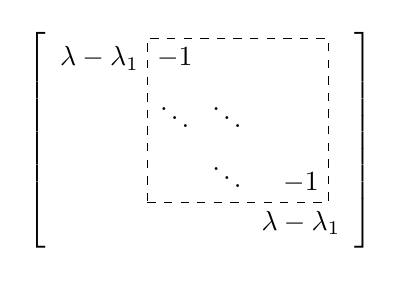
\begin{tikzpicture}[baseline=(math-axis),every right delimiter/.style={xshift=-3pt},every left delimiter/.style={xshift=3pt}]%
\matrix [matrix of math nodes,left delimiter={[},right delimiter={]}] (matrix)
{
|(m11)| \lambda-\lambda_1 & |(m12)| -1 & |(m13)| & |(m14)|\\
|(m21)| & |(m22)| \ddots & |(m23)| \ddots & |(m24)| \\
|(m31)| & |(m32)| & |(m33)| \ddots & |(m34)| -1\\
|(m41)| & |(m42)| & |(m43)| & |(m44)| \lambda-\lambda_1\\
};
\node[draw,dashed,inner sep=0pt,fit=(m12) (m14) (m32) (m34)] {};
\coordinate (math-axis) at ($(matrix.center)+(0em,-0.25em)$);
\end{tikzpicture}.
\]
As this submatrix is lower triangular, its determinant is equal to the product of its diagonal entries. The determinant of such matrices is therefore \(\pm 1\). As \(1\) and \(-1\) have only one monic common divisor, which is \(1\), one concludes that $\delta_k\big(P(\lambda)\big)=1$ for $k\in\{1,\dots,n-1\}$.
From~\eqref{eq:mgcdrecurse}, one can deduce that $d_k(\lambda)=1$ for $k\in\{1,\dots,n-1\}$.

When $k=n$, the only possible submatrix to consider is the whole matrix, whose determinant is equal to the product of the diagonal entries, $(\lambda-\lambda_1)^n$. One can deduce that $\delta_n\big(P(\lambda)\big)=(\lambda-\lambda_1)^n$.
Applying~\eqref{eq:mgcdrecurse} then yields $d_n(\lambda)=(\lambda-\lambda_1)^n$.
\end{proof}

\subsection*{A4}
Let $J_1 \in \complex^{n_1 \times n_1}$ and $J_2 \in \complex^{n_2 \times n_2}$ be two Jordan blocks with respective eigenvalues $\lambda_i$ and sizes $n_i$, $i = 1,2$. Let $A\in \complex^{n\times n}$ with $n = n_1+n_2$ be the Jordan matrix consisting of the two Jordan blocks $J_1$ and $J_2$. Then $\lambda I - A$ can be reduced to the form
\[
M(\lambda)(\lambda I-A)N(\lambda) = \diag\{\underbrace{1, \dots , 1}_{n_1 - 1 \textnormal{ times}}, (\lambda - \lambda_1)^{n_1}, \underbrace{1, \dots, 1}_{n_2 - 1 \textnormal{ times}}, (\lambda - \lambda_2)^{n_2}\},
\]
with unimodular matrices  $M(\lambda)$, $N(\lambda) \in \complex^{n\times n}[\lambda]$.

\begin{proof}
From A3, one knows that $P_i(\lambda) \triangleq \lambda I - J_i$ (for \(i = 1, 2\)) can be written as
\begin{align*}
P_i(\lambda) &\triangleq \lambda I_{n_i} - J_i\\
&= M_i(\lambda) D_i(\lambda) N_i(\lambda)\\
\iff D_i &= M_i^{-1}(\lambda)P_i(\lambda) N_i^{-1}(\lambda)\\
&= \begin{bmatrix}
1 & & & &\\
  &1& & &\\
  & &\ddots& &\\
  & & & 1& \\
  & & &  &(\lambda - \lambda_i)^{n_i}
\end{bmatrix}.
\end{align*}

Note that $M_i^{-1}(\lambda), N_i^{-1}(\lambda)$ are unimodular, as they are inverses of unimodular matrices.

Now, if one considers the diagonal matrix \(D(\lambda)\) formed by combining $D_1(\lambda)$ and $D_2(\lambda)$, one finds
\begin{align*}
D(\lambda) \triangleq
\begin{bmatrix}
D_1(\lambda) &\\
& D_2(\lambda)
\end{bmatrix} &= \begin{bmatrix}
1 & & & &&&&&\\
  &1& & &&&&&\\
  & &\ddots& &&&&&\\
  & & & 1& &&&&\\
  & & &  &(\lambda - \lambda_1)^{n_1}&&&&\\
  &&&&&1 & & & &\\
  &&&&&&1& & &\\
  &&&&&& &\ddots& &\\
  &&&&&& & & 1& \\
  &&&&&&& &  &(\lambda - \lambda_2)^{n_2}\\
\end{bmatrix}\\
&=\begin{bmatrix}
M_1^{-1}(\lambda)P_1(\lambda) N_1^{-1}(\lambda) &\\
& M_2^{-1}(\lambda)P_2(\lambda) N_2^{-1}(\lambda)
\end{bmatrix}\\
&=
\underbrace{\begin{bmatrix}
M_1^{-1}(\lambda) &\\
& M_2^{-1}(\lambda)
\end{bmatrix}}_{\triangleq M(\lambda)}
\underbrace{\begin{bmatrix}
P_1(\lambda) &\\
& P_2(\lambda)
\end{bmatrix}}_{\triangleq P(\lambda) = (\lambda I - A)}
\underbrace{\begin{bmatrix}
N_1^{-1}(\lambda) &\\
& N_2^{-1}(\lambda)
\end{bmatrix}}_{\triangleq N(\lambda)}.
\end{align*}

$M(\lambda)$ is unimodular as its determinant is the product of the determinants of $M_1^{-1}(\lambda)$ and $M_2^{-1}(\lambda)$, both of which are unimodular; the determinant of $M(\lambda)$ is equal to the product of two nonzero constants, which is also a nonzero constant.
Similarly, $N(\lambda)$ is also unimodular.
\end{proof}

\begin{remark}
This result can easily be extended to an arbitrary number of Jordan blocks \(m\).
\begin{align}
\label{a4}
\underbrace{\begin{bmatrix}
D_1(\lambda) & &\\
& \ddots &\\
& & D_m(\lambda)
\end{bmatrix} }_{\triangleq D(\lambda)}
&=
\underbrace{\begin{bmatrix}
M_1^{-1}(\lambda) & &\\
& \ddots &\\
& & M_m^{-1}(\lambda)
\end{bmatrix}}_{\triangleq M^{-1}(\lambda)}
\underbrace{\begin{bmatrix}
P_1(\lambda) & &\\
& \ddots &\\
& & P_m(\lambda)
\end{bmatrix}}_{\triangleq P(\lambda) = (\lambda I - A)}
\underbrace{\begin{bmatrix}
N_1^{-1}(\lambda) & &\\
& \ddots &\\
& & N_m^{-1}(\lambda)
\end{bmatrix}}_{\triangleq N^{-1}(\lambda)}.
\end{align}
\end{remark}
\begin{proof}
By induction, let us consider $A=\left[\begin{smallmatrix}
B & \\
 & J_p
\end{smallmatrix}\right]$, with $B \in \complex^{n\times n}$ a block diagonal matrix with $(p-1)$ Jordan blocks and $J_p\in \complex^{n_p\times n_p}$ the \(p\)-th Jordan block. 
The previous proof verifies the base case $p = 2$.

For $p > 2$, one assumes that
\begin{align*}
\underbrace{\begin{bmatrix}
D_1(\lambda) & &\\
& \ddots &\\
& & D_{p-1}
\end{bmatrix} }_{\triangleq D_{B}(\lambda)}
&=
\underbrace{\begin{bmatrix}
M_1^{-1}(\lambda) & &\\
& \ddots &\\
& & M_{p-1}^{-1}(\lambda)
\end{bmatrix}}_{\triangleq M_{B}^{-1}(\lambda)}
\underbrace{\begin{bmatrix}
P_1(\lambda) & &\\
& \ddots &\\
& & P_{p-1}(\lambda)
\end{bmatrix}}_{\triangleq P_{B}(\lambda) = (\lambda I - B)}
\underbrace{\begin{bmatrix}
N_1^{-1}(\lambda) & &\\
& \ddots &\\
& & N_{p-1}^{-1}(\lambda)
\end{bmatrix}}_{\triangleq N_{B}^{-1}(\lambda)}.
\end{align*}

Then, 
\begin{align*}
P \triangleq \lambda I - A &= \begin{bmatrix}
\lambda I - B & \\
& \lambda I - J_p 
\end{bmatrix}\\
&= \begin{bmatrix}
M_{B}(\lambda) D_{B}(\lambda) N_{B}(\lambda) & \\
& \lambda I - J_p
\end{bmatrix}\\
&= \begin{bmatrix}
M_{B}(\lambda) D_{B}(\lambda) N_{B}(\lambda) & \\
& M_{p}(\lambda) D_{p}(\lambda) N_{p}(\lambda)
\end{bmatrix}\\
&= \underbrace{\begin{bmatrix}
M_{B}(\lambda) & \\
& M_{p}(\lambda)
\end{bmatrix}}_{\triangleq M(\lambda)}\underbrace{\begin{bmatrix}
D_{B}(\lambda) & \\
& D_{p}(\lambda)
\end{bmatrix}}_{\triangleq D(\lambda)}\underbrace{\begin{bmatrix}
N_{B}(\lambda) & \\
& N_{p}(\lambda)
\end{bmatrix}}_{\triangleq N(\lambda)}.
\end{align*}
From the first equation to the second, the inductive hypothesis was used, and from the second to the third, one simply needs to apply the results of A3.
\end{proof}

Now, one can find the elementary polynomials of $P(\lambda) \triangleq (\lambda I - A)$. For that, the property proved in A1 applied to the Smith decomposition, that is, $\delta_k\big(P(\lambda)\big) = \delta_k\big(D(\lambda)\big)$, will be used.

Note that the diagonal matrix $D(\lambda)$ that we obtained here is not the same matrix as the diagonal matrix in the Smith normal form containing the elementary polynomials $d_i(\lambda)$ even if the notations can be misleading.

Using A1, it is clear that for $k = 1, 2, \dots, (n_1 + n_2 - 2)$, one can always choose a submatrix having only ones on its diagonal, which means that $\delta_k\big(P(\lambda)\big) = 1$. 

Note that for this proof, we don't consider submatrices with a determinant equal to zero as it is irrelevant in our search for the greatest common divisor.

By A2, one has that the monic $d_i(\lambda)$ are all equal to \(1\) for $i = 1, 2, \dots, (n_1 + n_2 - 2)$.


One then needs to distinguish two cases:
\begin{itemize}
\item When $\lambda_1 \neq \lambda_2$, the \((n_1 + n_2 - 1)\)-minors are \((\lambda - \lambda_1)^{n_1},(\lambda - \lambda_2)^{n_2},\) and \((\lambda - \lambda_1)^{n_1}(\lambda - \lambda_2)^{n_2}\).
Their gcd is \(\delta_{n_1 + n_2 - 1}\big(P(\lambda)\big) = 1\).
Using~\eqref{eq:mgcdrecurse}, one finds that \(d_{n_1 + n_2 - 1}(\lambda) = 1\).
Similarly, the only \((n_1 + n_2)\)-minor is \((\lambda - \lambda_1)^{n_1}(\lambda - \lambda_2)^{n_2}\), hence \(\delta_{n_1 + n_2}\big(P(\lambda)\big) = (\lambda - \lambda_1)^{n_1}(\lambda - \lambda_2)^{n_2}\).
Using the recursive formula of~\eqref{eq:mgcdrecurse}, one thus finds \(d_{n_1 + n_2}(\lambda) = (\lambda - \lambda_1)^{n_1}(\lambda - \lambda_2)^{n_2}\).
\item When $\lambda_1 = \lambda_2$, the \((n_1 + n_2 - 1)\)-minors are \((\lambda - \lambda_1)^{n_1}, (\lambda - \lambda_1)^{n_2}\), and \((\lambda - \lambda_1)^{n_1 + n_2}\), hence their gcd is \(\delta_{n_1 + n_2 - 1}\big(P(\lambda)\big) = (\lambda - \lambda_1)^{\min\{n_1, n_2\}}\).
Applying~\eqref{eq:mgcdrecurse} then yields that \(d_{n_1 + n_2 - 1}(\lambda) = (\lambda - \lambda_1)^{\min\{n_1, n_2\}}\).
Similarly, the only \((n_1 + n_2)\)-minor is \((\lambda - \lambda_1)^{n_1 + n_2}\), hence \(\delta_{n_1 + n_2}\big(P(\lambda)\big) = (\lambda - \lambda_1)^{n_1 + n_2}\).
Using~\eqref{eq:mgcdrecurse}, one can deduce that \(d_{n_1 + n_2}(\lambda) = (\lambda - \lambda_1)^{\max\{n_1, n_2\}}\).
\end{itemize}

We can observe that the minimal polynomial of $A$ is equal to $d_{n_1+n_2}(\lambda)$.

\begin{remark}
This result can also be extended to the general case where \(A\) has an arbitrary number of Jordan blocks.
\end{remark}

\begin{proof}
By induction, let us consider $A=\left[\begin{smallmatrix}
B & \\
 & J_p
\end{smallmatrix}\right]$, with $B \in \complex^{n\times n}$ a block diagonal matrix with $(p-1)$ Jordan blocks and $J_p\in \complex^{n_p\times n_p}$ the \(p\)-th Jordan block.
The base case $p = 2$ has already been proven.

For $p > 2$, assume that the minimal polynomial of $B$ is equal to the last elementary polynomial of $(\lambda I - B)$: $d_{n}^{B}(\lambda) = \prod_{i = 1}^k (\lambda - \lambda_i)^{n_i}$, with $\lambda_i$, $i= 1, \dots, k$, the distinct eigenvalues of \(A\) and $n_i$ the size of the largest Jordan block associated to the corresponding eigenvalue.

We know that
\begin{align*}
P(\lambda)\triangleq\lambda I - A 
&= \underbrace{\begin{bmatrix}
M_{B}(\lambda) & \\
& M_{p}(\lambda)
\end{bmatrix}}_{\triangleq M(\lambda)}\underbrace{\begin{bmatrix}
D_{B}(\lambda) & \\
& D_{p}(\lambda)
\end{bmatrix}}_{\triangleq D(\lambda)}\underbrace{\begin{bmatrix}
N_{B}(\lambda) & \\
& N_{p}(\lambda)
\end{bmatrix}}_{\triangleq N(\lambda)}.
\end{align*}

This means that $\delta_{n+n_p}\big(P(\lambda)\big) = \delta_{n+n_p}\big(D(\lambda)\big) = \prod_{i = 1}^p (\lambda - \lambda_i)^{n'_i}$ with $p$ the total number of Jordan blocks and $n'_i$ the size of each Jordan block.

As previously, we don't consider submatrices with a determinant equal to zero as it is irrelevant in our search for the greatest common divisor.

We must then consider two cases:
\begin{itemize}
\item If $\lambda_i \neq \lambda_p$, for all $i\neq p$, then $(\lambda - \lambda_p)^{n'_p}$ is not a divisor of any \(i\)-minor with $i < (n+n_p)$.
This means that $d_{n+n_p}(\lambda) = d_{n}^{B}(\lambda) (\lambda - \lambda_p)^{n'_p}$.
This corresponds to the minimal polynomial of \(A\).
\item If there exists $i \neq p$ such that $\lambda_p = \lambda_i$, then let us denote $y$ as the number of Jordan blocks with an eigenvalue equal to $\lambda_p$. It is clear that if one chooses any submatrix of dimension $(n+n_p-y+1)$, there will be at least one occurrence of $(\lambda - \lambda_p)^{z}$ in the diagonal terms used to compute the minor (with $z \in \mathcal{Z}_p$, $\mathcal{Z}_p$ being the set of all sizes of Jordan blocks with eigenvalue equal to $\lambda_p$).
This then means that $(\lambda - \lambda_p)^{\min(\mathcal{Z}_p)}$ must divide $\delta_{n+n_p-y+1}\big(P(\lambda)\big)$ and $d_{n+n_p-y+1}^{A}(\lambda)$.
This reasoning can be continued by considering  $\mathcal{Z}_p \setminus \min(\mathcal{Z}_p)$, and submatrices of dimension $(n+n_p-y+2)$, and so forth, continually removing the minimum in the set until one arrives at matrices of dimension $(n+n_p)$, where
\[
d_{n+n_p}^{A}(\lambda) = \frac{\delta_{n+n_p}\big(P(\lambda)\big)}{\prod_{z \in \mathcal{Z}_p\setminus \max{\mathcal{Z}_p}}(\lambda - \lambda_p)^{z}},
\]
which means that the only contribution of $\lambda_p$ to $d_{n+n_p}^{A}(\lambda)$ is $(\lambda - \lambda_p)^{\max(\mathcal{Z}_p)}$. One can then, from $d_{n+n_p}^{B}(\lambda)$, take out the factor with $\lambda_p$ in it, and replace it with the new $(\lambda - \lambda_p)^{\max(\mathcal{Z}_p)}$. With this, one obtains the minimal polynomial of \(A\).
\end{itemize}
The previous conclusion for \(p=2\) thus still holds in the general case.
\end{proof}

\subsection*{A5}
Let $A\in \complex^{n\times n}$. There are unimodular matrices $M(\lambda), N(\lambda) \in \complex^{n\times n}[\lambda]$ such that 
\[
\lambda I - A = M(\lambda)E(\lambda)N(\lambda),
\]
where $E(\lambda)$ is diagonal with its elements being either \(1\)'s or polynomials of the form $(\lambda - \lambda_i)^{n_i}$ where $\lambda_i$ are the eigenvalues of \(A\) and $n_i$ the size of the corresponding Jordan block in the Jordan decomposition of \(A\).

\begin{proof}
First, let us write the Jordan decomposition of \(A\).
\[
T^{-1} A T =J \iff A= T J T^{-1},
\]
with $J$ the Jordan matrix and $T$ a similarity transformation (this implies that $T$ is invertible, its determinant is nonzero, which means that it is a unimodular matrix).

One can then expand as follows:
\begin{align*}
\lambda I - A &= \lambda I - T J T^{-1}\\
&= T(\lambda I - J) T^{-1}\\
&= \underbrace{TM'(\lambda)}_{\triangleq M(\lambda)}\underbrace{D(\lambda)}_{\triangleq E(\lambda)}\underbrace{N'(\lambda)T^{-1}}_{\triangleq N(\lambda)},
\end{align*}
where the last equality is obtained with the results of A4,~\eqref{a4} in particular.
$M(\lambda)$ and $N(\lambda)$ are indeed unimodular as they are products of unimodular matrices.
\end{proof}

The matrices $A$ and $J$ have the same eigenvalues which means that they have the same minimal polynomial as well.
In A4, one could already observe that a Jordan matrix has a minimal polynomial equal to its last elementary polynomial.

The minimal polynomial of $A$ is thus equal to the last elementary polynomial of $\lambda I - J$ (obtained by studying $D(\lambda)$) which is also the last elementary polynomial of $\lambda I - A$ (obtained by studying $E(\lambda) = D(\lambda)$).

\section*{Exercise B: Implementation}
\subsection*{B1}
Using the Jordan normal form is not numerically stable because taking limits does not commute with forming the Jordan canonical form.
A simple example is the matrix \(A = I_2\), approximated by \(A_\varepsilon = \left[\begin{smallmatrix} 1 & \varepsilon \\ 0 & 1\end{smallmatrix}\right]\), the latter having Jordan canonical form \(J_\varepsilon = \left[\begin{smallmatrix} 1 & 1 \\ 0 & 1\end{smallmatrix}\right]\).
However, the Jordan form of \(A\) is simply \(J = I_2\).
We thus have
\[
\lim_{\varepsilon \to 0} A_\varepsilon = A, \quad \textnormal{but} \quad \lim_{\varepsilon \to 0} J_\varepsilon \neq J.
\]
Similarly, computing the minimal polynomials yields \(p_{A_\varepsilon}(\lambda) = (\lambda - 1)^2 \ne \lambda - 1 = p_A(\lambda)\).

\subsection*{B2}
We want to compute the Smith normal form of $P_i(\lambda) \triangleq \lambda I - A_{i}$ where $A_{i}$ is one of the three matrices $A_1$, $A_2$, and $A_3$ defined in the homework statement. The Smith normal forms are the following:
\begin{align*} P_1(\lambda) &=
    \begin{bmatrix}
    1 & 0 & 0 & 0 \\
    0 & 1 & 0 & 0 \\
    0 & 0 & 1 & 0 \\
    0 & 0 & 0 & \lambda^{4} + 4 \lambda^{3} + \frac{21 \lambda^{2}}{4} + \frac{11 \lambda}{4} + \frac{1}{2}
    \end{bmatrix}, \\
    P_2(\lambda) &=
    \begin{bmatrix}
    1 & 0 & 0 & 0 \\
    0 & 1 & 0 & 0 \\
    0 & 0 & 1 & 0 \\
    0 & 0 & 0 & \lambda^{4} + \frac{7 \lambda^{3}}{2} + \frac{7 \lambda^{2}}{2} + \lambda
    \end{bmatrix}, \\
    P_3(\lambda) &=
    \begin{bmatrix}
    1 & 0 & 0 & 0 \\
    0 & 1 & 0 & 0 \\
    0 & 0 & 1 & 0 \\
    0 & 0 & 0 & \lambda^{4} + 3 \lambda^{3} + 2 \lambda^{2}
    \end{bmatrix}.
\end{align*}

The minimal polynomial \(p_{A_i}(\lambda)\) of $A_{i}$ can be deduced from the last elementary polynomial of those Smith normal forms.
\begin{align*}
    \big(P_1(\lambda)\big)_{nn} &= \lambda^{4} + 4 \lambda^{3} + \frac{21 \lambda^{2}}{4} + \frac{11 \lambda}{4} + \frac{1}{2} \implies p_{A_1}(\lambda) = (\lambda + 1/2)^{2} (\lambda + 1) (\lambda + 2),\\
    \big(P_2(\lambda)\big)_{nn} &= \lambda^{4} + \frac{7 \lambda^{3}}{2} + \frac{7 \lambda^{2}}{2} + \lambda \implies p_{A_2}(\lambda) = \lambda (\lambda + 1/2) (\lambda + 1) (\lambda + 2),\\
    \big(P_3(\lambda)\big)_{nn} &= \lambda^{4} + 3 \lambda^{3} + 2 \lambda^{2}\vphantom{\frac{1}{1}} \implies p_{A_3}(\lambda) = \lambda^{2} (\lambda + 1) (\lambda + 2).
\end{align*}
If one wants to verify the boundednesss of the trajectories of the associated linear dynamical systems with transition matrices $A_1$, $A_2$ and $A_3$ defined in the homework statement, Statement~2 in the introduction of Exercise~A of Homework~3 is useful: ``All the eigenvalues of $A_{i}$ are in the open left-hand plane, or are on the imaginary axis and are simple.''
This statement has been shown to be equivalent to boundedness of trajectories.

To check whether this statement is satisfied or not, one must look at the vectors of eigenvalues $\Lambda_i$ of the matrices, which one can compute from the factorization of the minimal polynomial.
\begin{align*}
    \Lambda_1 =\begin{bmatrix}
    -1/2\\
    -1/2\\
    -1\\
    -2
    \end{bmatrix},\quad
    \Lambda_2 =\begin{bmatrix}
    0\\
    -1/2\\
    -1\\
    -2
    \end{bmatrix},\quad
    \Lambda_3 =\begin{bmatrix}
    0\\
    0\\
    -1\\
    -2
    \end{bmatrix}.
\end{align*}
One can observe that these eigenvalues are identical to the eigenvalues found for the third homework. The conclusion is thus similar: all eigenvalues of $A_1$ (for all \(i\)) are such that $\Re(\lambda_{1, i})<0$.
$A_1$ thus satisfies Statement~2, and has bounded trajectories.
The matrix $A_2$ has eigenvalues such that $\Re(\lambda_{2, i})<0$ for all \(i\) except for ($\lambda_{2, 1}=0$), which is simple (the multiplicity of this eigenvalue in the factorization of the minimal polynomial is one), so the statement is again verified, and the trajectories are bounded.
The matrix $A_3$ has eigenvalues ($\lambda_{3, 1} = \lambda_{3, 2} = 0$) with zero real part and with a multiplicity of two in the factorization of the minimal polynomial, which is not simple.
Therefore, it does not satisfy the statement and does not have bounded trajectories.
We conclude that only the first two systems have bounded trajectories, which is the same conclusion we arrived at in the previous homework.
\end{document}